
%(BEGIN_QUESTION)
% Copyright 2010, Tony R. Kuphaldt, released under the Creative Commons Attribution License (v 1.0)
% This means you may do almost anything with this work of mine, so long as you give me proper credit

Calculate $V_{BC}$, $V_{EH}$, and $V_{FG}$ in this four-wire RTD circuit, assuming the RTD transmitter uses a 0.35 mA current source to ``excite'' the RTD circuit:

$$\includegraphics[width=15.5cm]{i02316x01.eps}$$

Note: reference a {\it table} for this RTD to determine its resistance at the specified temperature.  

\vskip 10pt

Also, determine which of the four wires should be colored red, and which should be colored white.

\vskip 20pt \vbox{\hrule \hbox{\strut \vrule{} {\bf Suggestions for Socratic discussion} \vrule} \hrule}

\begin{itemize}
\item{} Does it matter to the accuracy of this system that the four wires have unequal resistances?
\item{} Which of the two requested voltages have the same value, and why?
\item{} When you look at the table of resistance values for a 10 ohm copper RTD, you will note it differs from platinum RTDs in terms of its ``10 ohm'' reference temperature.  What is the reference temperature for a 10 ohm copper RTD?
\end{itemize}

\underbar{file i02316}
%(END_QUESTION)





%(BEGIN_ANSWER)

$V_{BC}$ = 5.326 mV \hskip 30pt $V_{EH}$ = 5.326 mV \hskip 30pt $V_{FG}$ = 7.111 mV (calculations based on RTD table)

%(END_ANSWER)





%(BEGIN_NOTES)

An RTD table gives a resistance value of 15.217 ohms at 320 $^{o}$F.  The voltage $V_{BC}$ is simply the current source's value multiplied by this RTD resistance, equal to 5.326 mV.  The voltage $V_{EH}$ will be this exact same value, because the wires A-E and D-H are merely sensing wires and carry no current (therefore suffer no voltage drop across their lengths).

\vskip 10pt

The voltage drop $V_{FG}$ will be slightly larger, because wire resistance adds to RTD resistance to form a larger total resistance through which the 0.35 mA must flow.  The total resistance here is 20.317 ohms, yielding a voltage drop of 7.111 mV.

\vskip 10pt

As for wire colors, it doesn't matter so long as the colors match for wires that are connected to each other at the RTD.  For example: red wires at terminals A and B, and white wires at terminals C and D.





\vskip 20pt \vbox{\hrule \hbox{\strut \vrule{} {\bf Virtual Troubleshooting} \vrule} \hrule}

This question is a good candidate for a ``Virtual Troubleshooting'' exercise.  Presenting the diagram to students, you first imagine in your own mind a particular fault in the system.  Then, you present one or more symptoms of that fault (something noticeable by an operator or other user of the system).  Students then propose various diagnostic tests to perform on this system to identify the nature and location of the fault, as though they were technicians trying to troubleshoot the problem.  Your job is to tell them what the result(s) would be for each of the proposed diagnostic tests, documenting those results where all the students can see.

During and after the exercise, it is good to ask students follow-up questions such as:

\begin{itemize}
\item{} What does the result of the last diagnostic test tell you about the fault?
\item{} Suppose the results of the last diagnostic test were different.  What then would that result tell you about the fault?
\item{} Is the last diagnostic test the best one we could do?
\item{} What would be the ideal order of tests, to diagnose the problem in as few steps as possible?
\end{itemize}

%INDEX% Measurement, temperature: RTD (4-wire with cable resistance)

%(END_NOTES)

